\begin{frame}{Honeycomb Bosonic Mott Insulators}
\vskip-1.5cm
Does there exist a featureless bosonic insulator with charge 1 per unit cell on the honeycomb lattice?
%Is it possible to extend the Lieb Schultz Mattis theorem in this case
\only<1>{
\begin{columns}[T]
	\begin{column}[T]{.5\textwidth}
		\begin{figure}
			\scalebox{1}{
			%
% x=3*(minimum size)/2
% y=\sqrt{3/4}*(minimum size)/2
%

%http://tex.stackexchange.com/questions/6019/drawing-hexagons
\begin{tikzpicture}[x=7.5mm,y=4.33mm]
  % some styles
  \tikzset{
    box/.style={
      regular polygon,
      regular polygon sides=6,
      minimum size=10mm,
      inner sep=0mm,
      outer sep=0mm,
      rotate=0,
    draw
    }
  }
 \tikzset{boson/.style={circle=1pt,draw=black!100,fill=orange!100,inner sep=2pt}}

\foreach \i in {0,...,2} 
    \foreach \j in {0,...,3} {
            \node[box] at (2*\i,2*\j) {};
        }
\foreach \i in {0,...,1} 
    \foreach \j in {0,...,2} {
   	   \node[box] at (2*\i+1,2*\j+1) {};   
        }
\foreach \i in {0,...,2} 
    \foreach \j in {0,...,3} {
            \node[boson] at (2*\i-0.6,2*\j) {};
           % \node[boson] at (2*\i+0.6,2*\j) {};
           % \node[boson] at (2*\i-0.4,2*\j-1) {};
           % \node[boson] at (2*\i-0.4,2*\j+1) {};
             \node[boson] at (2*\i+0.4,2*\j+1) {};
              \node[boson] at (2*\i+0.4,2*\j-1) {};
        }
%\foreach \i in {0,...,1} 
  %  \foreach \j in {0,...,2} {
%	\node[boson] at (2*\i+1-0.6,2*\j+1) {}; 
%	\node[boson] at (2*\i+1+0.6,2*\j+1) {};   
   %   }
      
\end{tikzpicture}

			}\caption{Breaks rotational symmetry}
		\end{figure}
	\end{column}
	\begin{column}[T]{.5\textwidth}
		\begin{figure}
			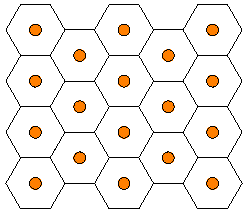
\includegraphics[width=.8\textwidth]{diagrams/hex_center_honeycomb.pdf}
			\caption{Leaves honeycomb lattice}
		\end{figure}
	\end{column}
\end{columns}
}
\only<2>{
\begin{figure}
\scalebox{1}{
% y=\sqrt{3/4}*(minimum size)/2
%

%http://tex.stackexchange.com/questions/6019/drawing-hexagons
\begin{tikzpicture}[x=7.5mm,y=4.33mm]
  % some styles
  \tikzset{
    box/.style={
      regular polygon,
      regular polygon sides=6,
      minimum size=10mm,
      inner sep=0mm,
      outer sep=0mm,
      rotate=0,
      dotted,
      thick,
      black,
      draw
    }
  }
 \tikzset{boson/.style={circle=1pt,draw=black!100,fill=orange!100,inner sep=2pt}}
  \tikzset{dimer/.style={ellipse=1pt,draw=black!100,fill=orange!90,inner sep=2pt}}
    \tikzset{thindimer/.style={ellipse=1pt,draw=black!100,fill=orange!90,inner sep=1pt}}

\foreach \i in {0,...,2} 
    \foreach \j in {0,...,3} {
            \node[box] at (2*\i,2*\j) {};
        }
\foreach \i in {0,...,1} 
    \foreach \j in {0,...,2} {
   	   \node[box] at (2*\i+1,2*\j+1) {};   
        }

 \foreach \i in {-1,...,2} 
     \foreach \j in {-1,...,2} 
     {
     \pgfmathtruncatemacro{\xa}{2*\i + 1*\j}
     \pgfmathtruncatemacro{\ya}{3*\j}
      \pgfmathtruncatemacro{\xb}{2*\i + 1*\j+1}
     \pgfmathtruncatemacro{\yb}{3*\j+1}
      \pgfmathtruncatemacro{\xc}{2*\i + 1*\j}
     \pgfmathtruncatemacro{\yc}{3*\j+2}
    
    \ifnum -1<\xa \ifnum \xa<5
     \ifnum\ya<7\ifnum-1<\ya 
	% \node[thindimer, rotate=120] at (\x-1/2,\y-1/2) {$\,\,\,\,$};     
     %\node[thindimer, rotate=120] at (\x+1/2,\y+1/2) {$\,\,\,\,$};
     %\node[thindimer, rotate=60] at (\x-1/2,\y+1/2) {$\,\,\,\,$};
       %\node[thindimer, rotate=60] at (\x+1/2,\y-1/2) {$\,\,\,\,$};
     \node[thindimer, rotate=0] at (\xa,\ya-1) {$\,\,\,\,$};
      \node[thindimer, rotate=0] at (\xa,\ya+1) {$\,\,\,\,$};
     \fi \fi\fi\fi
     
      \ifnum -1<\xc\ifnum \xc<5
     \ifnum \yc<7 \ifnum -2<\yc
       \node[thindimer, rotate=0] at (\xc,\yc+1) {$\,\,\,\,$};
       \fi\fi\fi \fi 
     }

\end{tikzpicture}
}
\caption{Breaks rotational symmetry}
\end{figure}}
\only<3>{
\begin{figure}
\scalebox{1}{
%
% x=3*(minimum size)/2
% y=\sqrt{3/4}*(minimum size)/2
%

%http://tex.stackexchange.com/questions/6019/drawing-hexagons
\begin{tikzpicture}[x=7.5mm,y=4.33mm]
  % some styles
  \tikzset{
    box/.style={
      regular polygon,
      regular polygon sides=6,
      minimum size=10mm,
      inner sep=0mm,
      outer sep=0mm,
      rotate=0,
    draw
    }
  }
 \tikzset{boson/.style={circle=1pt,draw=black!100,fill=orange!100,inner sep=2pt}}
  \tikzset{dimer/.style={ellipse=1pt,draw=black!100,fill=orange!90,inner sep=2pt}}

\foreach \i in {0,...,2} 
    \foreach \j in {0,...,3} {
            \node[box] at (2*\i,2*\j) {};
        }
\foreach \i in {0,...,1} 
    \foreach \j in {0,...,2} {
   	   \node[box] at (2*\i+1,2*\j+1) {};   
        }
% \foreach \i in {0,...,2} 
%     \foreach \j in {0,...,3} {
%     	  %\node[boson] at (2*\i-0.4,2*\j+1) {}; %TL of A hexagon
%          %\node[boson] at (2*\i+0.6,2*\j) {}; %R of A hexagon
%          %\node[boson] at (2*\i-0.4,2*\j-1) {}; %BL of A hexagon
% 
%          %\node[boson] at (2*\i-0.6,2*\j) {}; %L of  A hexagon
%          %\node[boson] at (2*\i+0.4,2*\j+1) {}; %TR of A hexagon
%          %\node[boson] at (2*\i+0.4,2*\j-1) {}; %BR of A hexagon
%         }
% \foreach \i in {0,...,1} 
%     \foreach \j in {0,...,2} {
% %	\node[boson] at (2*\i+1-0.6,2*\j+1) {}; %L of B hexagon
% %	\node[boson] at (2*\i+1+0.6,2*\j+1) {};   %R of B hexagon
%       }
 \foreach \i in {-1,...,2} 
     \foreach \j in {0,...,2} 
     {
     \pgfmathtruncatemacro{\x}{2*\i + 1*\j}
     \pgfmathtruncatemacro{\y}{3*\j}
     \ifnum
     -1<\x
     \ifnum
     \x<5
     \ifnum
     \y<7
     \ifnum
     -1<\y     
     \node[dimer, rotate=120] at (\x+1/2,\y+1/2) {$\,\,\,\,$};
     \node[dimer, rotate=60] at (\x-1/2,\y+1/2) {$\,\,\,\,$};
     \node[dimer, rotate=0] at (\x,\y-1) {$\,\,\,\,$};
     \fi
     \fi
     \fi
     \fi
     %\node[boson] at (\x, \y) {}; 
     }
    \node[dimer, rotate=120] at (0-1/2,3+1/2) {$\,\,\,\,$};
    \node[dimer, rotate=60] at (5-1/2,3+1/2) {$\,\,\,\,$};
      
\end{tikzpicture}
}
\caption{Breaks translationally symmetry, unit cell is 3 times larger}
\end{figure}}
\only<4>{
	\begin{columns}[T]
	\begin{column}[T]{0.5\textwidth}
		\begin{figure}
			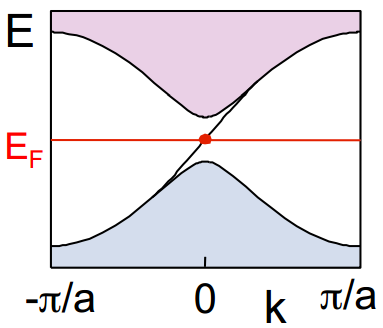
\includegraphics[width=0.5\linewidth]{diagrams/chiral_edge.png}
			\caption{Band insulator with chiral edge \footnotemark}
			%Not viewed as some integer number of orbitals filled per unit cell
		\end{figure}
	\end{column}
	\begin{column}[T]{0.5\textwidth}
		\begin{figure}
			\vskip-0.7cm
				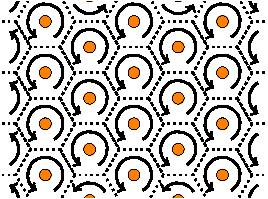
\includegraphics[width=0.5\linewidth]{diagrams/honeycomb_breakdown.pdf}
				\caption{}
		\end{figure}
	\end{column}
	\end{columns}
\footnotetext[1]{
\citep{Hasan2010-fq}}		
}
\only<5>{
\begin{columns}[T]
	\begin{column}[T]{.65\textwidth}
		\begin{figure}
		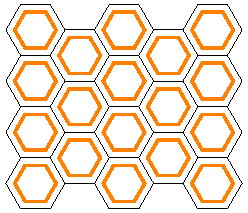
\includegraphics[width=.6\textwidth]{fbi3.pdf}
		\caption{Proposed Solution by \cite{kimchi2013}}
		\end{figure}
	\end{column}
	\begin{column}[T]{.35\textwidth}
	\begin{center}
					$$
\ket{\psi} = \prod\limits_{\varhexagon} \left(\sum\limits_{i \in \varhexagon} b^{\dagger}_i \right) \ket{\mathbf{0}}
			$$ 
	\end{center}
	\end{column}
\end{columns}
}

'Classical cartoons and usual tricks' lead to symmetry breaking, as noticed by \cite{parameswaran2013}

\end{frame}